\chapter{Moto del corpo rigido}
    Un corpo rigido è un modello per oggetti materiali indeformabili. Esso è formalmente un sistema di $n$ punti materiali obbedienti il \emph{vincolo di rigidità}
    \begin{equation}
        \|\x_j-\x_i\|=r_{i,j}=\mathrm{cost},\quad\forall i,j \in \{1,\dots,n\}.
    \end{equation}
    Un corpo rigido possiede al più $6$ gradi di libertà. Prendiamo a caso un punto $\x_1$ appartenente al corpo rigido. Per descriverne la posizione servono necessariamente 3 coordinate perché non abbiamo altri riferimenti. Un altro punto $\x_2$ del corpo rigido però sarà soggetto al vincolo $ \|\x_1-\x_2\|=r_{1,2}$, dunque ha $3-1=2$ gradi di libertà. Un terzo punto $\x_3$ invece sarà soggetto a due vincoli,  $\|\x_2-\x_3\|=r_{2,3}$ e $ \|\x_1-\x_3\|=r_{1,3}$, per cui avrà un solo grado di libertà. Ogni altro punto ha 0 gradi di libertà perché è soggetto a 3 vincoli, dunque la sua posizione sarà interamente determinata da $\x_1,\,\x_2,\,\x_3$ e dal vincolo di corpo rigido. Segue che il numero di gradi di libertà del sistema è quello del sistema $\x_1,\,\x_2,\,\x_3$, ovvero 6.
    \subsection{Cinematica del corpo rigido}
    Un sistema di riferimento $S'=(O',\hat{u}_1,\,\hat{u}_2,\,\hat{u}_3)$ è detto \emph{solidale} al corpo rigido se, rispetto ad esso, la velocità di ogni punto costituente il corpo rigido è nulla. In soldoni un sistema di riferimento è solidale se è ancorato al corpo rigido: esso ruota quando il corpo ruota, trasla quando il corpo trasla. È chiaro che la posizione dei punti che costituiscono il corpo rigido è sempre nota in $S'$, per cui il problema di descrivere la posizione del corpo rigido in un sistema inerziale $S=(O,\,\hat{e}_1,\,\hat{e}_2,\,\hat{e}_3)$ si riconduce a conoscere la posizione di $S'$, ovvero le $3$ coordinate dell'origine $O'$ e l'orientamento nello spazio di $\hat{u}_1,\,\hat{u}_2,\,\hat{u}_3$.
    
    Possiamo descrivere l'orientamento spaziale di $\hat{u}_1,\,\hat{u}_2,\,\hat{u}_3$ immaginando di traslare $O'\to O$ e osservando che $S'$ è una copia ruotata di $S$. Per far coincidere $S$ ed $S'$ basta ruotare $S$, l'entità e la direzione di questa rotazione descrive totalmente l'orientamento di $\hat{u}_1,\,\hat{u}_2,\,\hat{u}_3$ rispetto a $\hat{e}_1,\,\hat{e}_2,\,\hat{e}_3$.

    Per far coincidere $S$ ed $S'$ servono al più 3 rotazioni. Per prima cosa ruotiamo attorno a $\hat{e}_3$ di un angolo $\varphi$ in modo che 
    \begin{equation}
        (\hat{e}_1,\,\hat{e}_2,\,\hat{e}_3) \to (\hat{n},\hat{e}_2', \hat{e}_3).
    \end{equation}
    Questa trasformazione è descritta dalla matrice
    \begin{equation}
        A_1 = \begin{bmatrix}
            \cos \varphi & \sin \varphi & 0\\
            -\sin \varphi &\cos \varphi & 0 \\
            0 & 0 & 1
        \end{bmatrix}
    \end{equation}
    Infatti applicando $A_1$ a $\hat{e}_3=(0,0,1)$ vediamo che esso rimane invariato, mentre
    \begin{equation}
    \begin{aligned}
    &\hat{e}_1 \to  \cos \varphi \,\hat{e}_1 -\sin \varphi \,\hat{e}_2  =: \hat{n},\\
    &\hat{e}_2 \to \sin \varphi\,\hat{e}_1 +\cos \varphi\,\hat{e}_2 =: \hat{e}_2'.
    \end{aligned}
    \end{equation}
    Ora ruotiamo attorno a $\hat{n}$ di un angolo $\theta$ in modo che
    \begin{equation}
        (\hat{n},\hat{e}_2', \hat{e}_3) \to (\hat{n}, \hat{e}_2'', \hat{u}_3),
    \end{equation}
    questa trasformazione è descritta da:
    \begin{equation}
        A_2 = 
        \begin{bmatrix}
            1 & 0 & 0\\
            0 & \cos \theta & \sin \theta \\
            0 & -\sin \theta & \cos \theta
        \end{bmatrix}, 
    \end{equation}
    per cui i nuovi vettori sono
    \begin{equation}
    \begin{aligned}
        & \hat{n} = \hat{n}\\
        &\hat{e}_2'' = \cos \theta \,\hat{e}_2' -\sin \theta \,\hat{e}_3\\
        & \hat{u}_3 = \sin \theta \hat{e}_2'+\cos \theta \,\hat{e}_3.
    \end{aligned}
    \end{equation}
    L'ultima rotazione la facciamo attorno a $\hat{u}_3$ di un angolo $\psi$:
    \begin{equation}
    \begin{aligned}
        &(\hat{n}, \hat{e}_2'', \hat{u}_3) \to (\hat{u}_1,\,\hat{u}_2,\,\hat{u}_3)\\
        &A_3 = 
        \begin{bmatrix}
            \cos \psi & \sin \psi & 0\\
            -\sin \psi &\cos \psi & 0 \\
            0 & 0 & 1
        \end{bmatrix}\\
        &\hat{u}_1 = \cos \psi\,\hat{n}-\sin \psi\,\hat{e}_2''\\
        &\hat{u}_2 = \sin \psi\,\hat{n}+\cos \psi\,\hat{e}_2''\\
        &\hat{u_3} = \hat{u_3}.
    \end{aligned}
    \end{equation}
     Sostituendo opportunamente è possibile ricavare le espressioni dei vettori in termini della base iniziale. Vediamo quindi che i $3$ angoli $\varphi,\,\theta,\,\psi$, detti \emph{angoli di Eulero}, permettono di individuare l'orientamento della terna solidale rispetto alla terna fissa. 

    Importante nella descrizione del moto di un corpo rigido è il vettore \emph{velocità angolare} definito da
    \begin{equation}
        \w := \braket{\deriv \hat{u}_2 |\hat{u}_3}\hat{u}_1+\braket{\deriv \hat{u}_3 |\hat{u}_1}\hat{u}_2+\braket{\deriv \hat{u}_1 |\hat{u}_2}\hat{u}_3.
    \end{equation}
    Il motivo dell'importanza di questo vettore è nel seguente teorema:
    \begin{theorem}
        \textbf{Formula di Poisson}\\
        La derivata temporale del versore $u_k,\,k \in \{1,2,3\}$ del sistema di riferimento $S' = (O',\hat{u}_1,\,\hat{u}_2,\,\hat{u}_3)$ è data da
        \begin{equation}
            \deriv \hat{u}_k = \w \times \hat{u}_k.
        \end{equation}
    \end{theorem}
    \begin{proof}
        Calcoliamo la derivata del versore $\hat{u}_1$.
        $\deriv \hat{u}_1$ è un vettore di $\R^3$ quindi 
        \begin{equation}
            \deriv \hat{u}_1 = \sum_k \lambda_k \hat{u}_k,
        \end{equation}
        essendo la base $\hat{u}_k$ ortonormale, i coefficienti sono la proiezione del vettore lungo ognuno degli assi:
        \begin{equation}
            \deriv \hat{u}_1 = \sum_{k=1}^3 \braket{\deriv \hat{u}_1|\hat{u}_k} \hat{u}_k
        \end{equation}
        Osserviamo che la derivata di un versore è sempre perpendicolare al versore stesso:
        \begin{equation}
            \deriv \braket{\hat{u}_1|\hat{u}_1} =2\braket{\deriv \hat{u}_1|\hat{u}_1}= \deriv 1 = 0 \iff \deriv \hat{u}_1 \perp \hat{u}_1,
        \end{equation}
        per cui la sommatoria si semplifica in 
        \begin{equation}
            \deriv \hat{u}_1 = \braket{\deriv \hat{u}_1| \hat{u}_2}\hat{u}_2 + \braket{\deriv \hat{u}_1| \hat{u}_3}\hat{u}_3.
        \end{equation}
        e che il prodotto vettoriale tra $\hat{u}_1$ e $\w$ è
        \begin{equation}
            \w \times \hat{u}_1 = \det 
            \begin{bmatrix}
                \hat{u}_1 &\hat{u}_2 & \hat{u}_3\\
                \omega_1 & \omega_2 & \omega_3 \\
                1 & 0 &0
            \end{bmatrix} = \omega_3 \hat{u}_2-\omega_2\hat{u}_3 = \braket{\deriv \hat{u}_1| \hat{u}_2}\hat{u}_2-\braket{\deriv \hat{u}_3|\hat{u}_1}\hat{u}_3.
        \end{equation}
        Ma i vettori della terna sono sempre ortogonali tra loro, ovvero $\braket{\hat{u}_3|\hat{u}_1}\equiv 0$, dunque
        \begin{equation}
            0= \deriv \braket{\hat{u}_3|\hat{u}_1} = \braket{\deriv \hat{u}_3| \hat{u}_1}+ \braket{\hat{u}_3|\deriv \hat{u}_1}
        \end{equation}
        da cui segue che
        \begin{equation}
            \braket{\deriv \hat{u}_3| \hat{u}_1} = -\braket{\hat{u}_3|\deriv \hat{u}_1}
        \end{equation}
        che dimostra la tesi.
    \end{proof}
    Qualsiasi vettore $\mathbf{v}$ che è fisso nella terna solidale, come ad esempio le posizioni $\r_i$ dei punti materiali che compongono il corpo rigido, può essere derivato moltiplicando per $\w$:
    \begin{equation}
    \begin{aligned}
        &\deriv \mathbf{v} = \deriv(\mathbf{v}_x\hat{u}_1+\mathbf{v}_y\hat{u}_2+\mathbf{v}_z\hat{u}_3) = \mathbf{v}_x\deriv \hat{u}_1+\mathbf{v}_y\deriv \hat{u}_2+\mathbf{v}_z\deriv \hat{u}_3= \\
        &=\mathbf{v}_x\w\wedge\hat{u}_1+\mathbf{v}_y\w\wedge \hat{u}_2+\mathbf{v}_z\w \wedge\,\hat{u}_3 = \w \wedge \mathbf{v},
    \end{aligned}
    \end{equation}
    però deve essere scritto in termini dei versori della terna solidale. Enunciamo anche un teorema fondamentale per le applicazioni che mette in relazione gli angoli di Eulero e la velocità angolare:

    \begin{theorem}
    \label{th: omega in eulero}
        Il vettore velocità angolare di una terna ortogonale può essere espressa come combinazione delle derivate degli angoli di Eulero nel seguente modo:
        \begin{equation}
            \w = \dot{\varphi}\hat{e}_3+\dot{\theta}\hat{n}+\dot{\psi}\hat{u}_3
            \label{omega in eulero}
        \end{equation}
        in termini di versori della terna solidale come:
        \begin{equation}
            \w = \hat{u}_1(\dot{\varphi}\sin\theta\sin\psi +\dot{\theta}\cos\psi)+\hat{u}_2(-\dot{\varphi}\sin\theta\cos\psi+\dot{\theta}\sin\psi)+\hat{u}_3(\dot{\psi}+\dot{\varphi}\cos\theta)
        \end{equation}
        e in termini di versori della terna fissa come:
        \begin{equation}
            \w = (\dot{\theta}\cos\varphi+\dot{\psi}\sin\varphi\sin\theta)\hat{e}_1+(\dot{\theta}\sin\varphi -\dot{\psi}\cos \varphi \sin \theta)\hat{e}_2+(\dot{\varphi}+\dot{\psi}\cos\theta)\hat{e}_3
        \end{equation}
    \end{theorem}
    \begin{proof}
        Per dimostrare la \ref{omega in eulero} consideriamo una rotazione attorno al solo $\hat{e}_3$ della terna solidale al corpo rigido, di entità $\varphi$ in senso anti orario. La trasformazione associata a tale rotazione è data dalla matrice
        \begin{equation}
            A = \begin{bmatrix}
                \cos \varphi & -\sin \varphi &0\\
                \sin\varphi &\cos\varphi & 0\\
                0 & 0 & 1
            \end{bmatrix}
        \end{equation}
        per cui i versori del sistema ruotato sono 
        \begin{equation}
        \begin{aligned}
            &\hat{u}_1 = A \hat{e}_1 =\cos \varphi \hat{e}_1+\sin\varphi\hat{e}_2\\
            &\hat{u}_2 = A \hat{e}_2 =-\sin \varphi \hat{e}_1+\cos\varphi\hat{e}_2\\
            &\hat{u}_3 = \hat{e}_3.
        \end{aligned}
        \end{equation}
        Si trova immediatamente che
        \begin{equation}
            \begin{aligned}
                &\omega_1 = \braket{\deriv \hat{u}_2|\hat{u}_3}=0\\
                &\omega_2 = \braket{\deriv \hat{u}_3|\hat{u}_1}=0.
            \end{aligned}
        \end{equation}
        mentre
        \begin{equation}
            \omega_3 = \braket{\deriv \hat{u}_1|\hat{u}_2} = \braket{-\dot{\varphi}\sin\varphi\hat{e}_1+\dot{\varphi}\cos\varphi \hat{e}_2|-\sin \varphi \hat{e}_1+\cos\varphi\hat{e}_2} = \dot{\varphi},
        \end{equation}
        dunque
        \begin{equation}
            \w = \dot{\varphi}\hat{u}_3=\dot{\varphi}\hat{e}_3.
        \end{equation}
        Considerando una rotazione attorno al solo $\hat{n}$ e poi attorno al solo $\hat{u}_3$ si ottengono le altri componenti del vettore $\w$ in termini di angoli di Eulero.

        Vediamo ora come il vettore $\w$ può essere scritto in termini dei versori della terna solidale. Partiamo dall'osservare che, secondo le rotazioni fatte sopra, 
        \begin{equation}
            \hat{u}_1 = A_3\hat{n},\, A_3 = 
        \begin{bmatrix}
            \cos \psi & \sin \psi & 0\\
            -\sin \psi &\cos \psi & 0 \\
            0 & 0 & 1
        \end{bmatrix}.
        \end{equation}
    
    segue che
    \begin{equation}
        \hat{n} = A_3^{-1}\hat{u}_1 = A_3^\dagger \hat{u}_1 = A_3 = 
        \begin{bmatrix}
            \cos \psi & -\sin \psi & 0\\
            \sin \psi &\cos \psi & 0 \\
            0 & 0 & 1
        \end{bmatrix} \begin{bmatrix}
            1\\
            0\\
            0
        \end{bmatrix} = \begin{bmatrix}
            \cos \psi\\
            \sin \psi\\
            0
        \end{bmatrix}
    \end{equation}
    Le componenti che abbiamo trovato per $\hat{n}$ sono nella base $\hat{u}_k$, per cui
    \begin{equation}
        \hat{n} = \cos \psi \hat{u}_1 +\sin\psi \hat{u}_2.
    \end{equation}
    Facciamo la stessa cosa per $\hat{e}_3$. Prima di tutto osserviamo che $\hat{u}_3 = A_2\hat{e}_3$, poi ricordiamo che dopo l'azione di $A_2$ la base è $\hat{n},\hat{e}_2'',\hat{u}_3$:
    \begin{equation}
        \hat{e}_3 = A_2^\dagger\hat{u}_3 = -\sin\theta \hat{e}''_2+\cos\theta \hat{u}_3,
    \end{equation}
    per cui ci rimane da esprimere $\hat{e}''_2$ in termini di $\hat{u}_k$. Ma $\hat{u}_2=A_3\hat{e}''_2$, dunque
    \begin{equation}
        \hat{e}''_2 = A_3^\dagger \hat{u}_2 = \sin\psi \hat{u}_1+\cos\psi\hat{u}_2.
    \end{equation}
    Troviamo $\w$ sostituendo e sommando:
    \begin{equation}
        \begin{aligned}
            &\w = \dot{\varphi}\hat{e}_3+\dot{\theta}\hat{n}+\dot{\psi}\hat{u}_3 = \dot{\varphi}(-\sin\theta \hat{e}''_2+\cos\theta \hat{u}_3)+\dot{\theta}(\cos \psi \hat{u}_1 +\sin\psi \hat{u}_2)+\dot{\psi}\hat{u}_3=\\
            &=\dot{\varphi}(-\sin\theta (\sin\psi \hat{u}_1+\cos\psi\hat{u}_2) +\cos\theta \hat{u}_3)+\dot{\theta}(\cos \psi \hat{u}_1 +\sin\psi \hat{u}_2)+\dot{\psi}\hat{u}_3=\\
            &=\hat{u}_1(\dot{\varphi}\sin\theta\sin\psi +\dot{\theta}\cos\psi)+\hat{u}_2(-\dot{\varphi}\sin\theta\cos\psi+\dot{\theta}\sin\psi)+\hat{u}_3(\dot{\psi}+\dot{\varphi}\cos\theta)
        \end{aligned}
    \end{equation}
    Per esprimere $\w$ in termini di $\hat{e}_k$ bisogna fare la stessa cosa, ma ovviamente sostituendo tutto in funzione degli $\hat{e}_k$. Osserviamo anche che il passaggio per esprimere $\hat{e}_3$ si poteva fare in unico passaggio moltiplicando entrambe le matrici insieme.
\end{proof}


    
    \section{Quantità meccaniche dei corpi rigidi}
    \subsection{Momento angolare}
    Un sistema di punti materiali di massa totale $M$ e con punti di coordinate $\r_1,\,\dots,\,\r_n$ possiede un \emph{momento angolare}
    \begin{equation}
        \J_{\boldsymbol{\Omega}} = \sum_{i=1}^n m_i(\r_i-\boldsymbol{\Omega}) \wedge \dot{\r}_i,
    \end{equation}
    dove $\boldsymbol{\Omega}\in \R^3$ è il \emph{polo} di calcolo del momento. Scriviamo questa quantità in modo più significativo ipotizzando di avere a che fare con un corpo rigido e mettendo in $\Omega$ l'origine del sistema di riferimento solidale. Questo è fatto perché rende $\r_i-\boldsymbol{\Omega}$ la scrittura nel sistema di riferimento solidale del vettore $\r_i$, dunque si avrà
    \begin{equation}
        \deriv (\r_i-\boldsymbol{\Omega}) = \w\wedge(\r_i-\boldsymbol{\Omega}).
    \end{equation}
    Facciamo apparire $\r_i-\boldsymbol{\Omega}$ sommando e sottraendo la velocità di spostamento del polo $\dot{\boldsymbol{\Omega}}:$
    \begin{equation}
    \begin{aligned}
        &\J_{\boldsymbol{\Omega}} = \sum_{i=1}^nm_i(\r_i-\boldsymbol{\Omega}) \wedge (\dot{\r}_i-\dot{\boldsymbol{\Omega}}+\dot{\boldsymbol{\Omega}}) = \sum_{i=1}^nm_i(\r_i-\boldsymbol{\Omega})\wedge \dot{\boldsymbol{\Omega}}+ \sum_{i=1}^nm_i(\r_i-\boldsymbol{\Omega})\wedge (\dot{\r}_i-\dot{\boldsymbol{\Omega}})=\\
        &= M\sum_{i=1}^n\frac{m_i(\r_i-\boldsymbol{\Omega})}{M}\wedge \dot{\boldsymbol{\Omega}}+ \sum_{i=1}^nm_i(\r_i-\boldsymbol{\Omega})\wedge (\w \wedge (\r_i-\boldsymbol{\Omega}))=\\
        &=M(\G-\boldsymbol{\Omega})\wedge\dot{\boldsymbol{\Omega}}+\J_{\mathrm{rot}, \boldsymbol{\Omega}},
        \end{aligned}
    \end{equation}
    Vediamo quindi che un contributo al momento angolare è dato dall'eventuale velocità di spostamento del polo, mentre un secondo contributo è dato da $\J_{\mathrm{rot}, \boldsymbol{\Omega}}$. Nella pratica è bene scegliere $\boldsymbol{\Omega}$ in modo che il primo contributo si annulli, questo può essere fatto scegliendo $\boldsymbol{\Omega}=\G$ oppure in modo che risulti $\dot{\boldsymbol{\Omega}}=0.$ Lavoriamo ora su $\J_{\mathrm{rot},\boldsymbol{\Omega}}$:
    \begin{equation}
        \begin{aligned}
           &\J_{\mathrm{rot},\boldsymbol{\Omega}} = \sum_{i=1}^nm_i(\r_i-\boldsymbol{\Omega})\wedge [\w \wedge (\r_i-\boldsymbol{\Omega})] = \\
           &=\sum_{i=1}^nm_i\left[\|\r_i-\boldsymbol{\Omega}\|^2\w-\braket{\w|\r_i-\boldsymbol{\Omega}}(\r_i-\boldsymbol{\Omega})\right],
           \label{jrot}
        \end{aligned}
    \end{equation}
    dove si è usata l'identità $a\wedge b\wedge c = b\braket{a|c}-c\braket{a|b}$\footnote{qual è la differenza tra un famoso compositore tedesco e un taxi? È Bac[h] - cab!}. Chiamando $x_i,y_i,z_i$ le coordinate di $\r_i$ nel sistema di riferimento solidale, risulta $\|\r_i-\boldsymbol{\Omega}\|=x_i^2+y_i^2+z_i^2$, per cui la componente $\hat{u}_1$ di $\J_{\mathrm{rot},\boldsymbol{\Omega}}$ è
    \begin{equation}
    \begin{aligned}
        &J^x_{\mathrm{rot},\boldsymbol{\Omega}} = \sum_{i=1}^nm_i\left[(x_i^2+y_i^2+z_i^2)\omega_x-(x_i\omega_x+y_i\omega_y+z_i\omega_z)x_i\right]=\\
        &=\sum_{i=1}^n m_i \left[(y_i^2+z_i^2)\omega_x -x_iy_i\omega_y-x_iz_i\omega_z\right]
    \end{aligned}
    \end{equation}
    da cui ricaviamo che
    \begin{equation}
        \J_{\mathrm{rot},\boldsymbol{\Omega}} = I\w,\,I = \sum_{i=1}^n m_i
        \begin{bmatrix}
            y_i^2+z_i^2 & -x_iy_i & -x_iz_i\\
             -x_iy_i   & x_i^2+z_i^2 & -y_iz_i\\
              -x_iz_i & -y_iz_i &x_i^2+y_i^2
        \end{bmatrix}
    \end{equation}
    che è una matrice simmetrica detta \emph{tensore di inerzia}. La componente $\alpha,\beta$ del tensore è
    \begin{equation}
        I_{\alpha,\beta} = \sum_{i=1}^n m_i(\|r_i^2\|\delta_{\alpha,\beta}-r_{i,\alpha}r_{i,\beta}).
    \end{equation}
    Si noti che se si scrive il tensore in una terna non solidale al corpo esso diventa $I=I(t).$ 
    Concludiamo scrivendo la formula completa per il momento angolare di un corpo rigido: 
    \begin{equation}
        \J_{\boldsymbol{\Omega}} = M(\G-\boldsymbol{\Omega})\wedge \dot{\boldsymbol{\Omega}}+ I_{\boldsymbol{\Omega}}\w,
    \end{equation}
    scegliendo il polo di riferimento coincidente con il centro di massa si ha la formula molto più semplice
    \begin{equation}
        \J = I_\G\w.
    \end{equation}
    Il fatto che $I$ sia simmetrica implica che è diagonalizzabile tramite una matrice del gruppo ortogonale di $\R^3$. In soldoni esiste una terna ortogonale, solidale al corpo rigido, in cui il tensore di inerzia è diagonale. Per trovare questa terna si può partire da qualsiasi sistema di riferimento solidale e ruotarlo --- perché questo è ciò che fa una matrice del gruppo ortogonale --- fino a trovare la terna giusta. Gli assi che compongono la terna diagonalizzante sono detti \emph{assi principali di inerzia.}
    
    
\subsection{Energia cinetica}
    Consideriamo ora l'energia cinetica del corpo rigido:
    \begin{equation}
        T = \frac{1}{2}\sum_{i=1}^n m_i\|\dot{\r}_i\|^2 = \frac{1}{2}\sum_{i=1}^n m_i\|\dot{\boldsymbol{\Omega}}+\dot{\r}_i-\dot{\boldsymbol{\Omega}}\|^2 .
    \end{equation}
    Sfruttiamo di nuovo il fatto che $\r_i-\boldsymbol{\Omega}$ è la posizione del punto materiale nella terna solidale per derivare usando il teorema di Poisson:
    \begin{equation}
        \begin{aligned}
            &T = \frac{1}{2}\sum_{i=1}^n m_i\|\dot{\boldsymbol{\Omega}}+\w\wedge(\r_i-\boldsymbol{\Omega})\|^2 = \frac{1}{2}\sum_{i=1}^n m_i\braket{\dot{\boldsymbol{\Omega}}+\w\wedge(\r_i-\boldsymbol{\Omega})|\dot{\boldsymbol{\Omega}}+\w\wedge(\r_i-\boldsymbol{\Omega})}=\\
            &=\frac{1}{2}\sum_{i=1}^{3n}m_i\dot{\boldsymbol{\Omega}}^2+ m_i\|\w\wedge(\r_i-\boldsymbol{\Omega})\|^2 + 2m_i \braket{\dot{\boldsymbol{\Omega}}|\w\wedge(\r_i-\boldsymbol{\Omega)}} =\\
            &= \frac{M}{2}\dot{\boldsymbol{\Omega}}^2 + \frac{1}{2}\sum_{i=1}^n m_i\|\w\wedge(\r_i-\boldsymbol{\Omega})\|^2+ 2m_i \braket{\dot{\boldsymbol{\Omega}}|\w\wedge(\r_i-\boldsymbol{\Omega)}}.
        \end{aligned}
    \end{equation}
    Ora ci concentriamo sul secondo termine ricordando la proprietà
    \begin{equation}
        a\cdot b\wedge c = c\cdot a \wedge b
    \end{equation}
    identificando
    \begin{equation}
        \begin{aligned}
            &a = \w\\
            &b = \r_i-\boldsymbol{\Omega}\\
            &c = \w \wedge (\r_i-\boldsymbol{\Omega})   
        \end{aligned}
    \end{equation}
    si ottiene
    \begin{equation}
        \w\cdot[(\r_i-\boldsymbol{\Omega})\wedge(\w \wedge (\r_i-\boldsymbol{\Omega}) )] = (\w \wedge (\r_i-\boldsymbol{\Omega}) )\cdot[\w\wedge(\r_i-\boldsymbol{\Omega}) ] = \|\w\wedge(\r_i-\boldsymbol{\Omega})\|^2
    \end{equation}
    ma il pezzo $[(\r_i-\boldsymbol{\Omega})\wedge(\w \wedge (\r_i-\boldsymbol{\Omega}) )]$ che compare al primo membro è lo stesso che appariva in $\J_{\mathrm{rot},\boldsymbol{\Omega}}$ nell'equazione \eqref{jrot}, per cui
    \begin{equation}
        \frac{1}{2}\sum_{i=1}^n m_i\|\w\wedge(\r_i-\boldsymbol{\Omega})\|^2 = \frac{1}{2}\sum_{i=1}^n m_i\w\cdot[(\r_i-\boldsymbol{\Omega})\wedge(\w \wedge (\r_i-\boldsymbol{\Omega}) )] = \frac{1}{2}\braket{\w|I\w}.
    \end{equation}
    L'ultimo pezzo della sommatoria può essere scritto in modo più significativo portando la sommatoria nel prodotto scalare:
    \begin{equation}
       \sum_i m_i \braket{\dot{\boldsymbol{\Omega}}|\w\wedge(\r_i-\boldsymbol{\Omega)}} = \braket{\dot{\boldsymbol{\Omega}}|\w\wedge\left(\sum_i m_i \r_i-\boldsymbol{\Omega}\right)} = M\braket{\dot{\boldsymbol{\Omega}}|\w\wedge(\G-\boldsymbol{\Omega})},
    \end{equation}
    da cui segue
    \begin{equation}
        T = \frac{M}{2}\dot{\boldsymbol{\Omega}}^2 + \frac{1}{2}\braket{\w|I\w} + M\braket{\dot{\boldsymbol{\Omega}}|\w\wedge(\G-\boldsymbol{\Omega})}.
    \end{equation}
    Scegliendo $\boldsymbol{\Omega}=\G$ si ottiene il \emph{Teorema di K\"onig per l'energia cinetica}:
    \begin{equation}
        T= \frac{M}{2}\dot{\G}^2 + \frac{1}{2}\braket{\w|I\w}.
    \end{equation}

   \section{Studio di una trottola pesante con punta fissa}
   Una trottola è un corpo rigido che è simmetrico rispetto a due assi ($\hat{u}_1$ e $\hat{u}_2$).
   \begin{center}
   \begin{tikzpicture}
    \node[below] at (0,-0.1){O};  
    \draw[name path=ellipse 1] (3.5,0) arc (0:360:3.5cm and 2cm);
    \draw[name path=ellipse 2,rotate=50] (3.5,0) arc (0:360:3.5cm and 2cm);
    \path [name intersections={of=ellipse 1 and ellipse 2}];
    \coordinate [] (A) at (intersection-4);
    
    \draw[very thick,-{latex}](0,0)--(0,3.5);
    \draw[](0,3.5)--(0,4)node[above]{$\hat{e}_3$};
    \node[]() at (85:3.5){$\dot{\varphi}$};
    \draw[shorten >=-1cm,very thick,-{latex}](0,0)--(A);
    \node[](x1) at (-65:3.5){$\hat{n}$};
    \node[] at (-75:3){$\dot{\theta}$};
    
    \draw[](0,0)--(-25:4.5)node[right]{$\hat{e}_2$};
    \draw[dash pattern=on 3mm off 3mm](0,0)--(-10:4.5)node[right](x2){$x^{'}$};
    \draw[dash pattern=on 3mm off 3mm](0,0)--(65:4.5)node[above]{$y^{'}$};
    \draw[-latex,thick](0,0)--(55:4.5)node[above]{$\hat{u}_2$};
    \draw[-latex](0,0)--(225:4.5)node[below left]{$\hat{e}_1$};
    \draw[-latex](0,0)--(135:4.5)node[above]{$\hat{u}_3$};
    \node[] at (135:5){$\dot{\psi}$};
    \node[] at (130:5){$z'$};
    
    %Arcs
    % x to x'
    %\coordinate (x1) at (-65:2);
    \coordinate (O) at (0,0);
    %\coordinate (x2) at (-10:2);
    \draw    pic [-latex,draw,angle radius=0.7cm] {angle = x1--O--x2};    
    \node[] at (0.8,-0.7){$\psi$};
    
    % y to y'
    \coordinate (y1) at (55:2);
    \coordinate (O) at (0,0);
    \coordinate (y2) at (65:2);
    \draw    pic [-latex,draw,angle radius=1.75cm] {angle = y1--O--y2};    
    
    % Z to z
    \coordinate (y1) at (90:2);
    \coordinate (O) at (0,0);
    \coordinate (y2) at (135:2);
    \draw    pic [-latex,draw,angle radius=3.0cm] {angle = y1--O--y2};    
    \node[] at (-1.5,3){$\theta$};
    
    % X to x
    \coordinate (y1) at (225:2);
    \coordinate (O) at (0,0);
    \coordinate (y2) at (-65:2);
    \draw    pic [-latex,draw,angle radius=0.7cm] {angle = y1--O--y2};    
    \node[] at (0,-1){$\varphi$};
    
    \draw[<-,rotate=-35,thick] (0.15,3.8) arc (-60:250:3.4mm and 1.25mm);
    \node[]at (50:4.25){$\omega_{y}$};
    
    \draw[<-,rotate=45,thick] (0.15,4) arc (60:-250:3.4mm and 1.25mm);
    \node[]at (130:4.2){$\omega_{z}$};
    
    %Wx
    \draw[->,thick] (-62:3) arc (-30:250:3mm and 3mm);
    \node[right] at (-60:3){$\omega_{x}$};
    %Rod of Spinner
    \draw[thick,rotate=45] (0,0)--(60:0.2)|-(90:0.95);
    \draw[thick,rotate=45] (0,0)--(120:0.2)|-(90:0.95);
    
    % draw spinner
    \coordinate (P) at (-1.3,1.3);% top of spinner
    \begin{scope}[shift={(0.3,-0.3)}, rotate around={-5:(-1,1)},
      every circle/.style={x={(1cm,0.8cm)},y={(0cm,1cm)}}] 
    % compute offset to tangent point
    \path[name path=ellipse 3] (0,0) circle[x radius=0.5, y radius=.5];
    \path[name path=radial 1] (0,0) -- (55:1);
    \path [name intersections={of=ellipse 3 and radial 1}];
    \coordinate (edge) at (intersection-1);
    
    \draw[fill=white,thick] (-0.9,0.9) circle[x radius=0.5,y radius=0.5];
    \draw[fill=white,thick] (-1,1) circle[x radius=0.5,y radius=0.5];
    \draw[thick] ($(-0.9,0.9)+(edge)$) -- ($(-1,1)+(edge)$)
                 ($(-0.9,0.9)-(edge)$) -- ($(-1,1)-(edge)$);% barely visible
    
    \coordinate (edge) at ($(0,0)!0.2!(edge)$);
    \draw[thick] (-1,1) circle[x radius=0.1,y radius=0.1];
    \fill[white] ($(P)+(edge)$) -- ($(-1,1)+(edge)$) -- ($(-1,1)-(edge)$) -- ($(P)-(edge)$) --  cycle;
    \draw[thick] ($(P)+(edge)$) -- ($(-1,1)+(edge)$) ($(-1,1)-(edge)$) -- ($(P)-(edge)$);
    \draw[thick] (P) circle[x radius=0.1,y radius=0.1];
    \end{scope}
    \draw[thick,-latex](0,0)--(135:3);
    
    \end{tikzpicture}
    \end{center}
%%%%%%%%%%%%%%%%%%%%%%%%%%%%%%%%%%%%%%%%%%%%%%%%%%%%%%%%%%%%%%%%%%%   
   
   Supponendo che la punta sia fissa nello stesso punto $O$, il suo moto è interamente descritto dai $3$ angoli di Eulero. Il moto della trottola pesante, ovvero soggetta a gravità, può essere descritto in 3 moti contemporanei:
   \begin{enumerate}
       \item Rotazione attorno all'asse $\hat{u}_3$ con velocità angolare $\dot{\psi}$.
       \item Precessione attorno all'asse $\hat{e}_3$ con velocità angolare $\dot{\varphi}$.
       \item Nutazione attorno all'asse $\hat{n}$ con velocità angolare $\dot{\theta}$.
   \end{enumerate}
    La velocità angolare è combinazione di questi 3 contributi:
    \begin{equation}
    \begin{aligned}
        &\boldsymbol{\omega} = \dot{\theta}\hat{n}+ \dot{\varphi}\hat{e}_3 + \dot{\psi}\hat{u}_3=\\
        &=\hat{u}_1(\dot{\varphi}\sin\theta\sin\psi +\dot{\theta}\cos\psi)+\hat{u}_2(-\dot{\varphi}\sin\theta\cos\psi+\dot{\theta}\sin\psi)+\hat{u}_3(\dot{\psi}+\dot{\varphi}\cos\theta)
    \end{aligned}
    \end{equation}
    per quanto già visto nel teorema \ref{th: omega in eulero}. Fissiamo $\Omega = O=(0,0,0)$ e, usando l'espressione dell'energia cinetica che abbiamo ricavato poco fa, troviamo
    \begin{equation}
        T = \frac{1}{2}\braket{\w|I\w} = \frac{I_1}{2}\w_1^2 +\frac{I_2}{2}\w_2^2+\frac{I_3}{2}\w_3^2 = \frac{I_1}{2}(\w_1^2+\w_2^2)+\frac{I_3}{2}\w_3^2,
    \end{equation}
    dove si è usato il tensore in forma diagonalizzata e nell'ultimo passaggio si è sfruttata la simmetria della trottola, che implica $I_1=I_2.$ Per fare questo è fondamentale esprimere la velocità angolare in termini dei versori $\hat{u}_k$, altrimenti il tensore dipenderebbe dal tempo e non sarebbe garantita la sua diagonalizzabilità. Chiamando $l$ la distanza del centro di massa da $O$, troviamo che
    \begin{equation}
        V = Mgl\cos\theta
    \end{equation}
    per cui 
    \begin{equation}
        \lag = \frac{I_1}{2}(\dot{\varphi}^2\sin^2\theta+\dot{\theta}^2)+\frac{I_3}{2}(\dot{\psi}+\dot{\varphi}\cos\theta)^2-Mgl\cos\theta.
    \end{equation}
    A questo punto si tratta di un esercizio già noto. Vediamo che $\psi,\varphi$ sono coordinate cicliche, che il sistema quindi è integrabile perché ha 3 gradi di libertà ($\psi,\theta,\varphi$) e 3 integrali primi ($p_\psi,p_\varphi, \ham$). Possiamo ricondurci ad un problema unidimensionale in $\theta$:
    \begin{equation}
    \begin{aligned}
        &P_\psi = I_3(\dot{\psi}+\dot{\varphi}\cos\theta)=:Ia\\
        &P_\varphi = I_1\dot{\varphi}\sin^2\theta+I_3(\dot{\psi}+\dot{\varphi}\cos\theta)\cos\theta=I_1\dot{\varphi}\sin^2\theta+Ia\cos\theta=:Ib
        \label{trottLagr}
    \end{aligned}
    \end{equation}
    dove $I=I_1=I_2$ e $a,b$ sono due costanti. Risolvendo la seconda equazione per $\dot{\varphi}$ otteniamo
    \begin{equation}
        \dot{\varphi} = \frac{b-a\cos\theta}{\sin^2\theta}.
    \end{equation}
    Sostituiamo tutto nell'energia $E=T+V$ per ottenere 
    \begin{equation}
        E = \frac{I}{2}\dot{\theta}^2+\frac{I}{2}\frac{\left(b-a\cos\theta\right)^2}{\sin^2\theta}+\frac{I^2a^2}{2I_3}+Mgl\cos\theta
    \end{equation}
    Assorbiamo la costante $\frac{I^2a^2}{2I_3}$ nella definizione del potenziale:
    \begin{equation}
         E = \frac{I}{2}\dot{\theta}^2+\frac{I}{2}\frac{\left(b-a\cos\theta\right)^2}{\sin^2\theta}+Mgl\cos\theta
    \end{equation}
    vediamo ora che il moto in $\theta$ è determinato dal potenziale efficace
    \begin{equation}
      V= \frac{I}{2}\frac{\left(b-a\cos\theta\right)^2}{\sin^2\theta}+Mgl\cos\theta.
    \end{equation}
    La situazione non è semplice a causa dei $\sin\theta$ e $\cos\theta$ che appaiono, tuttavia possiamo semplificare il tutto introducendo $u=\cos\theta\implies\dot{u} = -\dot{\theta}\sin\theta$ e sostituendo nell'energia:
    \begin{equation}
        \begin{aligned}
            &E =\frac{I}{2}\frac{\dot{u}^2}{\sin^2\theta} +\frac{I}{2}\frac{(b-au)^2}{\sin^2\theta}+Mglu\\
            &E\sin^2\theta = \frac{I}{2}\dot{u}^2 + \frac{I}{2}(b-au)^2+Mglu\sin^2\theta\\
            &\frac{I}{2}\dot{u}^2+\frac{I}{2}(b-au)^2+(Mglu-E)(1-u^2)=0\\
            & \dot{u}^2 +(b-au)^2+(\beta u-\alpha)(1-u^2)=0,
        \end{aligned}
    \end{equation}
    dove $\beta = 2Mgl/I$ e $\alpha = 2E/I.$
    Il nuovo potenziale efficace è
    \begin{equation}
        V^* = (b-au)^2+(\beta u-\alpha)(1-u^2).
    \end{equation}
    Si vede che $V^*(\pm\infty)=\mp\infty$ e che $V^*(\pm1)>0$. Noi siamo interessati alla regione $[-1,+1]$ perché $u$ è un coseno.
    \begin{figure}[h]
        \centering
        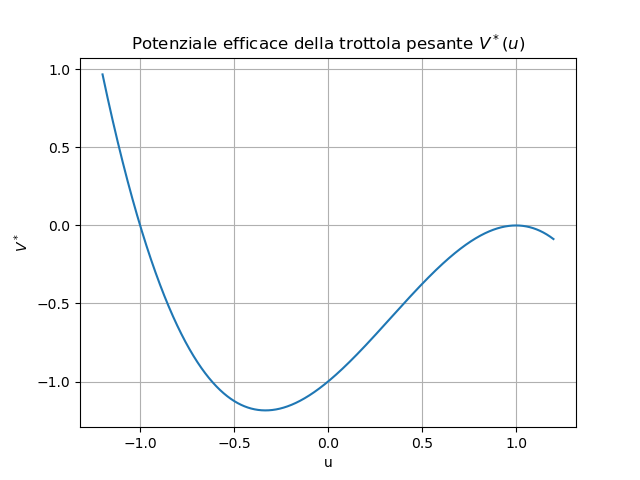
\includegraphics[width=0.7\linewidth]{img/trottola_pesante.png}
        \caption{Potenziale efficace della trottola pesante.}
        \label{fig:enter-label}
    \end{figure}
    Vediamo quindi che i moti in $\theta$ sono sempre periodici o, al più, di equilibrio stabile. Il periodo del moto in $\theta$ è detto \emph{periodo di nutazione} della trottola e si trova con la solita formula
    \begin{equation}
        T_\theta = \int_{u_-}^{u_+}\frac{\de u}{\sqrt{-(1-u^2)(\beta u - \alpha)-(b-au)^2}}
    \end{equation}
    Se $b>a$ allora $\dot{\varphi}>0 \,\forall t$ e il moto in $\varphi$ risulta sinusoidale. Se $b=a$ allora quando $u=\pm1$ $\dot{\varphi}=0$ e quindi $\varphi$ presenta delle cuspidi in $u=1$. Se $b<-1$ allora $\dot{\varphi}$ cambia di segno e quindi la traiettoria di $\varphi(\theta)$ è una curva non semplice, ovvero con delle auto intersezioni\footnote{Grafici presi da \url{https://mathcurve.com/courbes3d.gb/feston/feston.shtml}}:

    \begin{figure}[H]
    \centering
    \begin{minipage}[b]{0.3\linewidth}
        \centering
        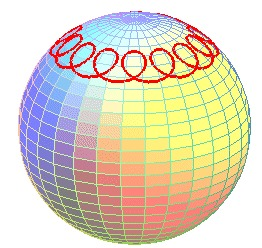
\includegraphics[width=\linewidth]{img/intersezioni.jpeg}
    \end{minipage}
    \hfill
    \begin{minipage}[b]{0.3\linewidth}
        \centering
        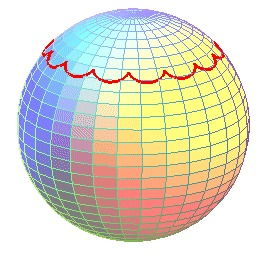
\includegraphics[width=\linewidth]{img/cuspidi.jpeg}
    \end{minipage}
    \hfill
    \begin{minipage}[b]{0.3\linewidth}
        \centering
        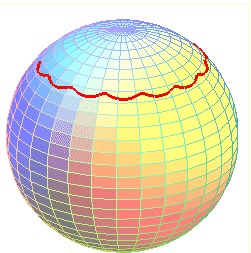
\includegraphics[width=\linewidth]{img/normale.jpeg}
    \end{minipage}
    \caption{Grafici di $\varphi$ in funzione di $\theta$ al variare di $a,b$.}
\end{figure}


    
    \subsection{Trottola dormiente}
    Una trottola dormiente è una trottola verticale che non nuta, ovvero in cui $\theta\equiv0$. Dalla seconda equazione delle \ref{trottLagr}, sostituendo $\theta=0$, si ottiene $a=b$. Questo semplifica l'energia:
    \begin{equation}
        \begin{aligned}
            &\dot{\varphi} = a\frac{1-\cos\theta}{\sin^2\theta}\\
            &E = \frac{I}{2}\dot{\theta}^2+\frac{I}{2}a^2\frac{(1-\cos\theta)^2}{\sin^2\theta}+Mgl\cos\theta
        \end{aligned}
    \end{equation}
    Chiaramente se $\dot{\theta}$ rimanesse nullo $E$ sarebbe mal definita in questa forma, però possiamo usare questa espressione per capire se lo stato di trottola dormiente è stabile o instabile considerando $\theta$ piccoli. Espandendo intorno a $\theta_0=0$ in Taylor si vede che
    \begin{equation}
        \frac{(1-\cos\theta)^2}{\sin^2\theta} =\frac{ (-\theta/2)^2}{\theta^2} +\dots \sim \frac{\theta^4}{4\theta^2}+\dots
    \end{equation}
    mentre
    \begin{equation}
        Mgl\cos\theta = Mgl-\frac{Mgl}{2}\theta^2+ O(\theta^4),
    \end{equation}
    dunque assorbendo la costante abbiamo
    \begin{equation}
        V = \theta^2\left[\frac{Ia}{4}-\frac{Mgl}{2}\right].
    \end{equation}
    Il potenziale della trottola dormiente tende ad una parabola per $\theta$ piccoli. La domanda ora è se il punto $\theta=0$ sia stabile oppure no, ovvero quale sia la concavità della parabola. Ricordiamo però dalla prima delle \ref{trottLagr} che $Ia$ dipende dalla velocità di rotazione $\dot{\psi}$, per cui è chiaro che la stabilità dipenda dalla velocità di rotazione della trottola. Nel caso di $\dot{\psi}$ molto grandi (caso di \emph{trottola veloce}) il punto sarà stabile, altrimenti instabile.

    \section{Equazioni cardinali e di Eulero}
    Deriviamo il momento angolare rispetto al tempo per ottenere la seconda equazione cardinale:
    \begin{equation}
        \deriv \J_{\boldsymbol{\Omega}} = \deriv(M(\G-\boldsymbol{\Omega})\wedge \dot{\boldsymbol{\Omega}})+ \deriv I\w.
    \end{equation}
    Bisogna stare attenti nella derivazione di $I\w$ perché in questa formula i vettori sono espressi come combinazione lineare dei versori $\hat{u}_k$, per cui
    \begin{equation}
        \deriv \w = \deriv \sum_{k=1}^3 \omega_k \hat{u}_k = \sum_{k=1}^3 \dot{\omega}_k\hat{u}_k + \omega_k\deriv \hat{u_k} = \sum_{k=1}^3 \dot{\omega}_k\hat{u}_k +\omega_k\wedge\hat{u}_k.
    \end{equation}
    Segue che
    \begin{equation}
        \deriv I\w = I\dot{\w}+\w\wedge I\w
    \end{equation}
    mentre
    \begin{equation}
        \deriv(M(\G-\boldsymbol{\Omega})\wedge \dot{\boldsymbol{\Omega}}) = M\dot{\G}\wedge\dot{\boldsymbol{\Omega}} + M(\G-\boldsymbol{\Omega})\wedge\ddot{\boldsymbol{\Omega}},
    \end{equation}
    per cui abbiamo
    \begin{equation}
        \deriv J_{\boldsymbol{\Omega}} = M\dot{\G}\wedge\dot{\boldsymbol{\Omega}} + M(\G-\boldsymbol{\Omega})\wedge\ddot{\boldsymbol{\Omega}} + I\dot{\w}+\w\wedge I\w.
    \end{equation}
    D'altra parte possiamo anche calcolare la derivata del momento angolare con la definizione:
    \begin{equation}
        \J_{\boldsymbol{\Omega}} = \sum_i m_i(\r_i-\boldsymbol{\Omega})\wedge\dot{\r}_i \implies \deriv \J_{\boldsymbol{\Omega}} = \sum_i m_i\deriv(\r_i-\boldsymbol{\Omega})\wedge\dot{\r}_i + \boldsymbol{\tau}_{\boldsymbol{\Omega}},
    \end{equation}
    dove
    \begin{equation}
        \boldsymbol{\tau}_{\boldsymbol{\Omega}} = \sum_{i=1}^{3n}m_i(\r_i-\boldsymbol{\Omega})\wedge\ddot{\r}_i
    \end{equation}
    è il momento torcente complessivo agente sul corpo. La derivata di $\r_i-\boldsymbol{\Omega}$ rispetto al tempo si semplifica:
    \begin{equation}
        \sum_i m_i\deriv(\r_i-\boldsymbol{\Omega})\wedge\dot{\r}_i = \sum_i m_i \dot{\r}_i\wedge \dot{\r_i} -\sum_i m_i\dot{\boldsymbol{\Omega}}\wedge\dot{\r}_i =-M\dot{\boldsymbol{\Omega}}\wedge \dot{\G}
    \end{equation}
    eguagliando le due espressioni si ottiene
    \begin{equation}
       - M\dot{\boldsymbol{\Omega}}\wedge \dot{\G}+\boldsymbol{\tau}_{\boldsymbol{\Omega}} = M\dot{\G}\wedge\dot{\boldsymbol{\Omega}} + M(\G-\boldsymbol{\Omega})\wedge\ddot{\boldsymbol{\Omega}} + I\dot{\w}+\w\wedge I\w
    \end{equation}
    per cui, in ultimo e ricordando l'antisimmetria del prodotto vettoriale:
    \begin{equation}
        \boldsymbol{\tau}_{\boldsymbol{\Omega}}=M(\G-\boldsymbol{\Omega})\wedge\ddot{\boldsymbol{\Omega}} + I\dot{\w}+\w\wedge I\w,
    \end{equation}
    \emph{seconda equazione cardinale.}

    Possiamo derivare le equazioni di Eulero dalla seconda equazione cardinale mettendoci nel caso $\boldsymbol{\tau}_{\boldsymbol{\Omega}}=0$. Questa situazione corrisponde ad esempio ad un solido su cui non agiscono forze, come un solido libero nello spazio. Prendiamo anche $\G = \boldsymbol{\Omega}$ in modo da semplificare l'equazione in
    \begin{equation}
        I\dot{\w}+\w\wedge I\w =0.
    \end{equation}
    Prendiamo anche il tensore diagonalizzato, in modo che sia facile esplicitare questa equazione differenziale per ogni componente del vettore $\w = \sum_{k=1}^3 \omega_k\hat{u}_k$:
    \begin{equation}
        \begin{cases}
            \dot{\omega}_1 = \frac{I_2-I_3}{I_1}\omega_2\omega_3\\
            \dot{\omega}_2 = \frac{I_3-I_1}{I_2}\omega_1\omega_3\\
            \dot{\omega}_3 = \frac{I_1-I_2}{I_3}\omega_1\omega_2
        \end{cases}
    \end{equation}
    I punti di equilibrio del sistema si ottengono mettendo $\dot{\w}=0$ e sono:
    \begin{equation}
        \begin{aligned}
            &\w = (\omega,0,0)\\
            &\w = (0,\omega,0)\\
            &\w = (0,0,\omega).
        \end{aligned}
    \end{equation}
    \subsection{Trottola libera}
    Abbiamo visto che la simmetria della trottola implica $I_1=I_2=I$, che trasforma le equazioni di Eulero in
    \begin{equation}
        \begin{cases}
            \dot{\omega}_1 = \frac{I-I_3}{I}\omega_2\omega_3\\
            \dot{\omega}_2 = \frac{I_3-I}{I}\omega_1\omega_3\\
            \dot{\omega}_3 = 0
        \end{cases}
    \end{equation}
    dunque $\omega_3=\mathrm{cost}$ e, derivando
    \begin{equation}
        \begin{cases}
            \ddot{\omega}_1 = \frac{I-I_3}{I}\dot{\omega}_2\omega_3\\
            \ddot{\omega}_2 = \frac{I_3-I}{I}\dot{\omega}_1\omega_3\\
        \end{cases}
    \end{equation}
    possiamo sostituire $\dot{\omega}_2$ e $\dot{\omega}_1$ dal sistema precedente per avere
    \begin{equation}
        \begin{cases}
            \ddot{\omega}_1 = \frac{I-I_3}{I}\frac{I_3-I}{I}\omega_1\omega^2_3\\
            \ddot{\omega}_2 = \frac{I_3-I}{I}\frac{I-I_3}{I}\omega_2\omega^2_3\\
        \end{cases} \iff
        \begin{cases}
            \ddot{\omega}_1 = -\left(\omega_3\frac{I-I_3}{I}\right)^2\omega_1\\
            \ddot{\omega}_2 = -\left(\omega_3\frac{I-I_3}{I}\right)^2\omega_2\\
        \end{cases}
    \end{equation}
    per cui il sistema ha soluzioni
    \begin{equation}
        \begin{cases}
            \omega_1(t) = A_1\cos(rt+\varphi_1)\\
            \omega_2(t) = A_2\cos(rt+\varphi_2)\\
            \omega_3 = \mathrm{cost}
        \end{cases},\quad r=\omega_3\frac{I-I_3}{I}
    \end{equation}
    Possiamo anche interpretare questo sistema fisico alla luce degli angoli di Eulero scrivendone la Lagrangiana, che è uguale a quella del caso di trottola con punta fissa ma ovviamente senza il potenziale delle forze:
    \begin{equation}
        \lag = \frac{I}{2}(\dot{\varphi}^2\sin^2\theta+\dot{\theta}^2)+\frac{I_3}{2}(\dot{\psi}+\dot{\varphi}\cos\theta)^2
    \end{equation}
    dunque abbiamo sempre gli integrali primi $p_\psi,\,p_\varphi$, inoltre l'ipotesi di momento delle forze nullo assicura la conservazione del momento angolare $\J_{\boldsymbol{\Omega}}$ in modulo, direzione e verso. Scegliamo $\hat{e}_3$ in modo che quello sia il versore del momento angolare e sia $k$ il modulo. Scriviamo il momento angolare nella base solidale con il solito cambio di base del teorema \ref{th: omega in eulero}:
    \begin{equation}
    \J = kA_3^\dagger A_2^\dagger\hat{e}_3
        \begin{bmatrix}
            \cos\psi &-\sin\psi &0\\
            \sin\psi &  \cos\psi&0\\
            0 & 0 & 1
        \end{bmatrix}\begin{bmatrix}
            1 & 0 & 0\\
            0 & \cos \theta & -\sin\theta \\
            0 & \sin \theta & \cos \theta
        \end{bmatrix}\begin{bmatrix}
            0\\
            0\\
            k
        \end{bmatrix}=\begin{bmatrix}
            \sin\psi \sin \theta k\\
           - \cos\psi\sin\theta k\\
            \cos\theta k
        \end{bmatrix} = \begin{bmatrix}
            I\omega_1\\
            I\omega2\\
            I_3\omega_3
        \end{bmatrix}
        \label{questaDZHANI}
    \end{equation}
    da cui si evince $\theta=\mathrm{cost}$, ovvero assenza di nutazione. Dai momenti coniugati si può invece ricavare $\dot{\varphi}=\mathrm{cost}$ e $\dot{\psi}=\mathrm{cost}$, dunque
    \begin{equation}
        \psi(t) = \psi_0+\dot{\psi}t,\quad\varphi(t) = \varphi_0+\dot{\varphi}t, \quad \theta = \theta_0.
    \end{equation}
    \subsection{Effetto Dzhanibekov (Teorema dell'asse intermedio)}
    Riprendiamo le equazioni di Eulero, ma consideriamo ora il caso di un solido asimmetrico libero. Senza perdere in generalità supponiamo $I_1<I_2<I_3$. Abbiamo imparato che per studiare i sistemi fisici conviene solitamente usare gli integrali primi invece di risolvere l'equazione, e sappiamo che a causa dell'assenza di momenti esterni è sia il momento angolare sia l'energia a conservarsi. In particolare essendo nulla la forza a cui è soggetto il solido la conservazione dell'energia coincide con la conservazione dell'energia cinetica. Si ha quindi
    \begin{equation}
        \begin{aligned}
            &T = \sum_{k=1}^3 \frac{I_k}{2}\omega_k^2 =\mathrm{cost}\\
            &\J = I\w =\mathrm{cost}    
        \end{aligned}
    \end{equation}
    $\J$ è costante in modulo, direzione e verso, dunque in particolare
    \begin{equation}
        \|J\|^2 = \sum_{k=1}^3 I_k^2\omega_k^2 =\mathrm{cost} .
    \end{equation}
    Vediamo anche che
    \begin{equation}
        T = \frac{J^2_1}{2I_1}+\frac{J^2_2}{2I_2}+\frac{J^2_3}{2I_3}=\mathrm{cost},
    \end{equation}
    dunque nello spazio $(J_1,\,J_2,\,J_3)$ l'energia cinetica rappresenta un ellissoide, mentre $J_1^2+J_2^2+J_3^2-\|J\|^2=0 $ è una sfera di raggio $\|J\|$. Se un corpo ha energia cinetica $T$ e momento angolare di modulo $\|J\|$, allora poiché queste quantità si conservano il suo moto dovrà sempre avvenire sull'intersezione tra l'ellissoide dell'energia cinetica e la sfera del momento angolare:
    \begin{figure}[H]
        \centering
        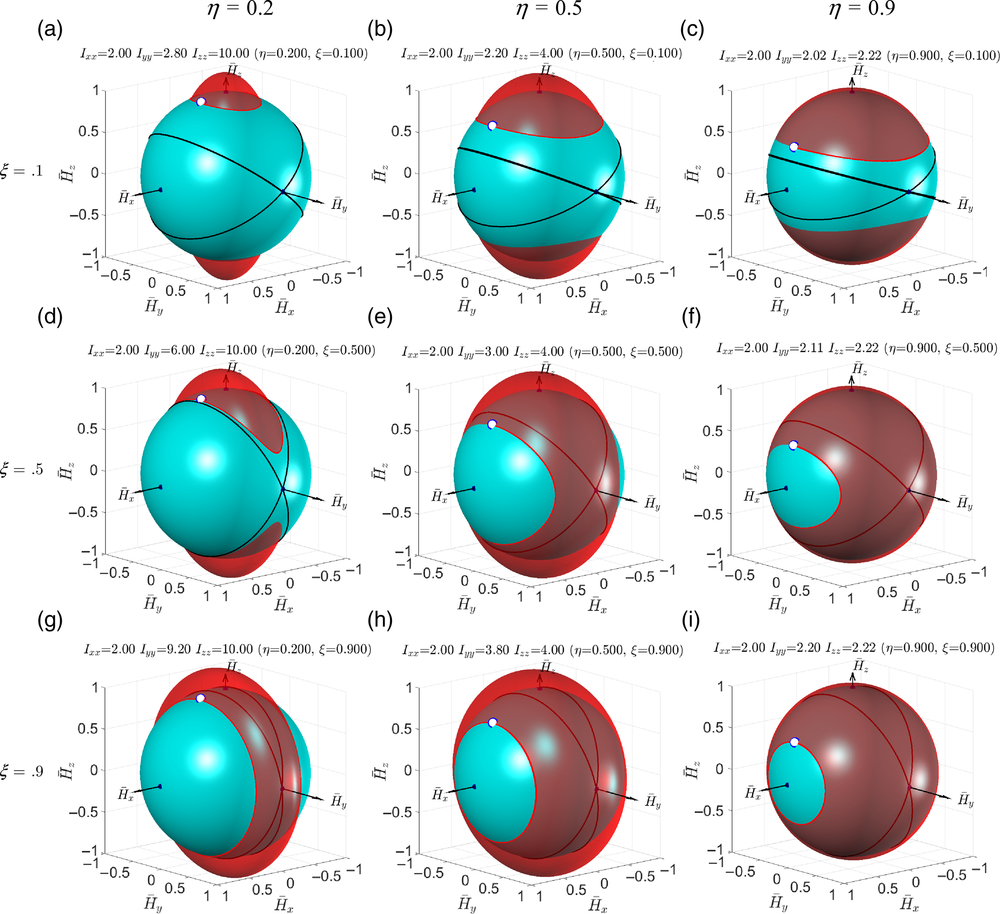
\includegraphics[width=0.9\linewidth]{img/dzhani.png}
        \caption{Intersezioni tra l'ellissoide cinetico e la sfera del momento angolare}
        \label{fig:placeholder}
    \end{figure}

    Con "effetto Dzhanibekov" ci si riferisce all'instabilità di rotazioni effettuate lungo l'asse intermedio $I_2$. Una rotazione che parte lungo il solo asse con momento di inerzia $I_2$ tende a trasformarsi in una rotazione che coinvolge anche gli altri assi. Possiamo studiare la stabilità dell'asse intermedio riconducendo il tutto a un "moto" unidimensionale. Definiamo due costanti $\lambda^2$ e $I$ tali che:
    \begin{equation}
        \begin{cases}
            \lambda^2 = I_1\omega_1^2+I_2\omega_2^2+I_3\omega_3^2\\
            \lambda^2I = I_1^2\omega_1^2+I_2^2\omega_2^2+I_3^2\omega_3^2
        \end{cases}
    \end{equation}
    risolvendo la prima equazione per $\omega_1^2$ otteniamo
    \begin{equation}
        \omega_1^2 = \frac{\lambda^2-I_2\omega_2^2-I_3\omega_3^2}{I_1}
        \label{omega1}
    \end{equation}
    sostituendo nella seconda si ha
    \begin{equation}
        \lambda^2I = I_1\lambda^2-I_1I_2\omega_2^2-I_1I_3\omega_3^2+I^2_2\omega_2^2+I^2_3\omega_3^2
    \end{equation}
    dunque
    \begin{equation}
        \lambda^2(I-I_1) =I_2(I_2-I_1)\omega_2^2 + I_3(I_3-I_1)\omega_3^2 
    \end{equation}
    da cui possiamo ottenere $\omega_3^2$:
    \begin{equation}
        \omega_3^2 = \frac{\lambda^2(I_1-I)}{I_3(I_1-I_3)}-\frac{I_2(I_1-I_2)}{I_3(I_1-I_3)}\omega_2^2.
        \label{omega3}
    \end{equation}
    Sostituendo possiamo eliminare $\omega_3^2$ da \eqref{omega1}:
    \begin{equation}
        \omega_1^2 = \frac{\lambda^2(I_3-I)}{I(I_3-I_1)}-\frac{I_2(I_3-I_2)}{I_1(I_3-I_1)}\omega_2^2
        \label{omega1fine}
    \end{equation}
    sostituendo \eqref{omega1fine} e \eqref{omega3} nell'equazione di Eulero di $\omega_2$ otteniamo
    \begin{equation}
        \dot{\omega}_2 = \frac{I_3-I_1}{I_2}\sqrt{\frac{\lambda^2(I_3-I)}{I(I_3-I_1)}-\frac{I_2(I_3-I_2)}{I_1(I_3-I_1)}\omega_2^2}\sqrt{\frac{\lambda^2(I-I_1)}{I_3(I_3-I_1)}-\frac{I_2(I_2-I_1)}{I_3(I_3-I_1)}\omega_2^2.}
    \end{equation}
    Semplifichiamo l'espressione raccogliendo i termini costanti davanti a $\omega_2^2$:
    \begin{equation}
        \dot{\omega}_2 =\frac{I_3-I_1}{I_2}\sqrt{\frac{I_1-I_2}{I_1-I_3}\frac{I_2}{I_1} \frac{I_3-I_2}{I_3-I_1}\frac{I_2}{I_3}}\sqrt{(\omega_a^2-\omega_2^2)(\omega_b^2-\omega_2^2)},
    \end{equation}
    con
    \begin{equation}
        \omega_a^2 = \frac{\lambda^2(I_1-I)}{I_2(I_1-I_2)},\quad \omega_b^2=\frac{\lambda^2(I_3-I_2)}{I_2(I_3-I_2)}.
    \end{equation}
    A questo punto ci siamo ricondotti all'equazione $\dot{\omega}_2^2+V(\omega_2)$, di cui possiamo studiare la stabilità. Per $I=I_1$ il potenziale ha una forma parabolica, per $I\neq I_1$ invece ha forma a \emph{cappello messicano}. Ricordando le \eqref{questaDZHANI} troviamo che $\cos\theta,\,\tan\psi$ non sono costanti in generale, dunque il moto lungo l'asse intermedio risulta in generale instabile.
    